\documentclass[aspectratio=149]{beamer}

\usepackage{bm}
\usetheme{metropolis}           % Use metropolis theme
\title{Fixed-Mean Gaussian Processes for post-hoc Bayesian Deep Learning}
\date{\today}
\author{Luis Antonio Ortega Andrés\\
Simón Rodríguez Santana\\
Daniel Hernández Lobato\\}
\institute{Autonomous University of Madrid}
\usepackage[most]{tcolorbox}

\newtcolorbox{HighlightBoxFit}[1][]{%
   enhanced,
   hbox,
   %fontupper=\itshape,
   before    = \par\smallskip\centering,
   after     = \par,
   width     = 14cm,
   colback   = blue!5,
   colframe  = blue!40!white, 
   arc       = 4mm, 
   outer arc = 3.5mm, 
   #1}

\NeedsTeXFormat{LaTeX2e}
\usepackage{amsfonts}       % blackboard math symbols
\usepackage{amssymb,amsmath,amsthm}
\usepackage{braket}
\usepackage{booktabs} % for professional tables
\usepackage{tabularx}
\usepackage{multirow}

\usefonttheme{professionalfonts} % required for mathspec
\usepackage{mathspec}
\setsansfont[BoldFont={Fira Sans}]{Fira Sans Light}

\newcommand{\h}[1]{\color{orange}\textbf{#1}}

\DeclareMathOperator*{\argmax}{arg\,max}
\DeclareMathOperator*{\argmin}{arg\,min}

\colorlet{shadecolor}{gray!40}
\begin{document}
  \maketitle


    {\setbeamercolor{background canvas}{bg=white}
      \begin{frame}{}
        \begin{figure}
            \centering
            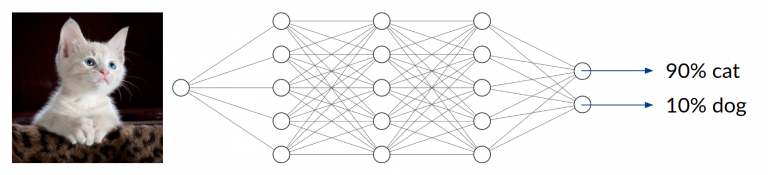
\includegraphics[width = 0.8\textwidth]{slides_imgs/Bildschirmfoto-vom-2019-10-01-11-03-08-768x175.png}
            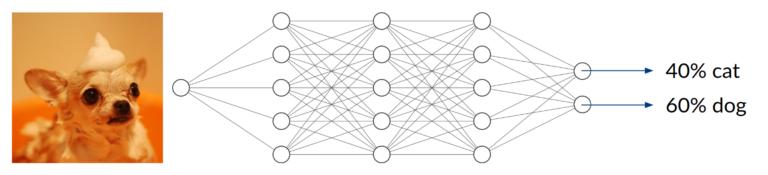
\includegraphics[width = 0.8\textwidth]{slides_imgs/uncertainty-quantification-dog-768x175.png}
        \end{figure}
    \end{frame}}
    
    {\setbeamercolor{background canvas}{bg=white}
      \begin{frame}{}
        \begin{figure}
            \centering
            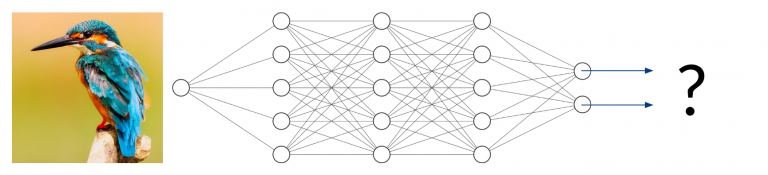
\includegraphics[width = 0.8\textwidth]{slides_imgs/Bildschirmfoto-vom-2019-10-01-11-03-18-768x175.png}
        \end{figure}
        \pause
        \begin{center}
        \textbf{Deep learning methods are unable to quantify the uncertainty of their predictions!}
        \end{center}
    \end{frame}}
    
    {\setbeamercolor{background canvas}{bg=white}
      \begin{frame}{}
      \textbf{Straight-forward solution}: Using a Bayesian model.
        \begin{figure}
            \centering
            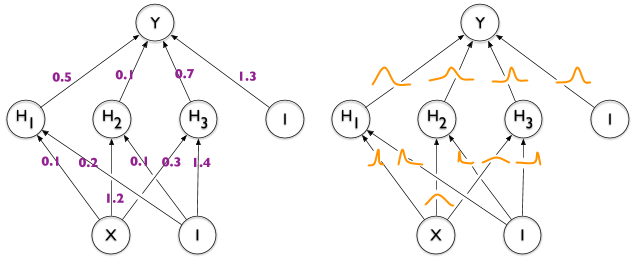
\includegraphics[width = 0.8\textwidth]{slides_imgs/Bayesian-Neural-Network.png}
        \end{figure}
    \end{frame}}

    \begin{frame}
        Making predictions \textbf{requires the posterior} over the parameters of the model \(\bm{\theta}\):
        \[
            p(y^\star | \mathbf{x}^\star, \mathcal{D}) = \int p(y^\star | \mathbf{x}^\star, \bm{\theta}) p(\bm{\theta} | \mathcal{D}) \ d\bm{\theta}\,,
        \]
        where \( p(\bm{\theta} | \mathcal{D}) \) is \textbf{intractable for complex models}.
    \end{frame}


    \begin{frame}
        \begin{center}
            Approximate  \( p(\bm{\theta} | \mathcal{D}) \) by something simpler \(q(\bm{\theta})\).
            \onslide<2>
            {
                \[
                    \Bigg\Downarrow
                \]
                \textbf{Poor performance in many cases.}
            }
        \end{center}
    \end{frame}

    \begin{frame}{Approach}

        \begin{enumerate}[<+->]
            \item Learn a DL \textbf{deterministic} model \(h\).
            \begin{center}
                \h{High Performance - No Uncertainty}
            \end{center}
            \item  Fixed-Mean Gaussian Processes with \textbf{posterior mean \(h\)}.
            \begin{center}
                \h{Same Performance - Uncertainty Estimation}
            \end{center}
            \item Optimize parameters using function-space VI.
        \end{enumerate}

    \end{frame}
        \begin{frame}{Gaussian Processes}
        \begin{center}\color{orange}
            \textbf{Uncertainty Estimation in function-space}
        \end{center}
        {\color{shadecolor}
        Given a mean \(m(\cdot)\) and covariance function \(K(\cdot, \cdot)\), defines a \textbf{Gaussian prior over function evaluations}:
        \[
        p(f(\mathbf{x})) = \mathcal{N}(m(\mathbf{x}), K(\mathbf{x}, \mathbf{x}))\,.
        \]
        \[
        f \sim \mathcal{G}\mathcal{P}(m, K)\,.
        \]
        }
    \end{frame}
    \begin{frame}{Gaussian Processes}
        \begin{center}\color{shadecolor}\textbf{Uncertainty Estimation in function-space}
        \end{center}
        {\color{black}
        Given a mean \(m(\cdot)\) and covariance function \(K(\cdot, \cdot)\), defines a {\color{orange}\textbf{Gaussian prior over function evaluations}}:
        \[
        p(f(\mathbf{x})) = \mathcal{N}(m(\mathbf{x}), K(\mathbf{x}, \mathbf{x}))\,.
        \]
        \[
        f \sim \mathcal{G}\mathcal{P}(m, K)\,.
        \]
        }
    \end{frame}
    \begin{frame}{Gaussian Processes}
    Set of observations \((\mathbf{X}, \mathbf{y})\), the \textbf{predictive distribution} is Gaussian
        \[
        p(y^\star | \mathbf{x}^\star, \mathbf{X}, \mathbf{y}) = \mathcal{N}(m^\star(\mathbf{x}^\star), K^\star(\mathbf{x}^\star, \mathbf{x}^\star))\,.
        \]
        \pause
        \[
        m^\star(\mathbf{x}^\star) = K(\mathbf{x}^\star, \mathbf{X})(K(\mathbf{X}, \mathbf{X}) + \sigma^2 \bm{I})^{-1}(\mathbf{y} - m(\mathbf{x}^\star))\,,
        \]
        \[
        K^\star(\mathbf{x}^\star, \mathbf{x}^\star) = K(\mathbf{x}^\star, \mathbf{x}^\star) - K(\mathbf{x}^\star, \mathbf{X})(K(\mathbf{X}, \mathbf{X}) + \sigma^2 \bm{I})^{-1}K(\mathbf{X},  \mathbf{x}^\star)\,.
        \]
        \begin{center}
            \emph{Gaussian noise with variance \(\sigma^2\) is considered for the targets}
        \end{center}
    \end{frame}

    \begin{frame}{Sparse Variational Gaussian Processes}
    \begin{center}
    Define a set of \emph{inducing locations} \(\mathbf{Z} \subset \mathbb{R}^D\) that ``summarize'' the training inputs \(\mathbf{X}\). 
    \end{center}

    \begin{center}
        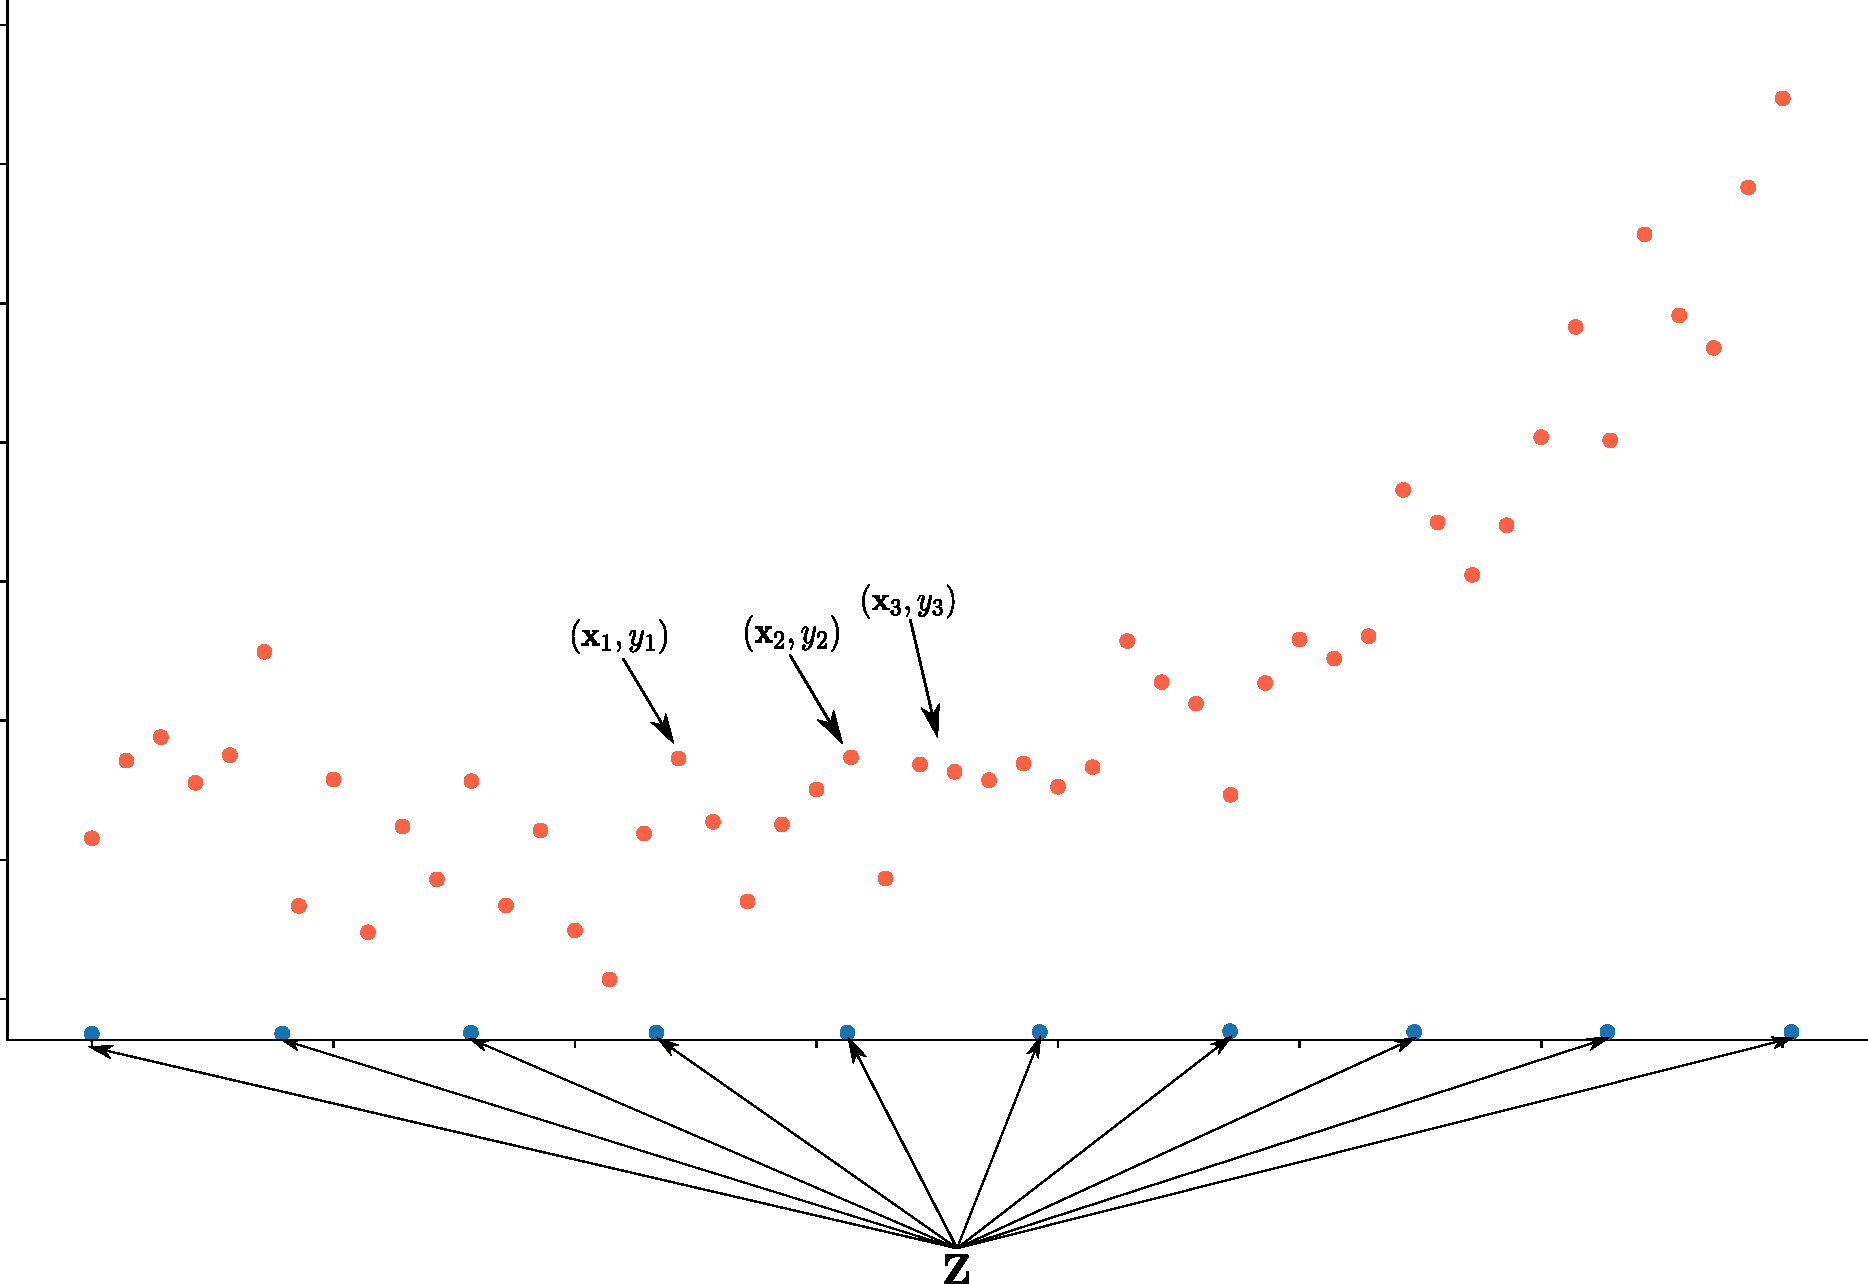
\includegraphics[width=0.7\textwidth]{slides_imgs/GP_inducing_1.pdf}
    \end{center}
    \end{frame}
    \begin{frame}{Sparse Variational Gaussian Processes}
    \begin{center}
    With \(\mathbf{u} = f(\mathbf{Z})\), the posterior \(p(\mathbf{u}|\mathbf{X}, \mathbf{y})\) is approximated with variational distribution \(q(\mathbf{u}) = \mathcal{N}(\bm{\mu}, \bm{\Sigma})\).
    \end{center}

    \begin{center}
        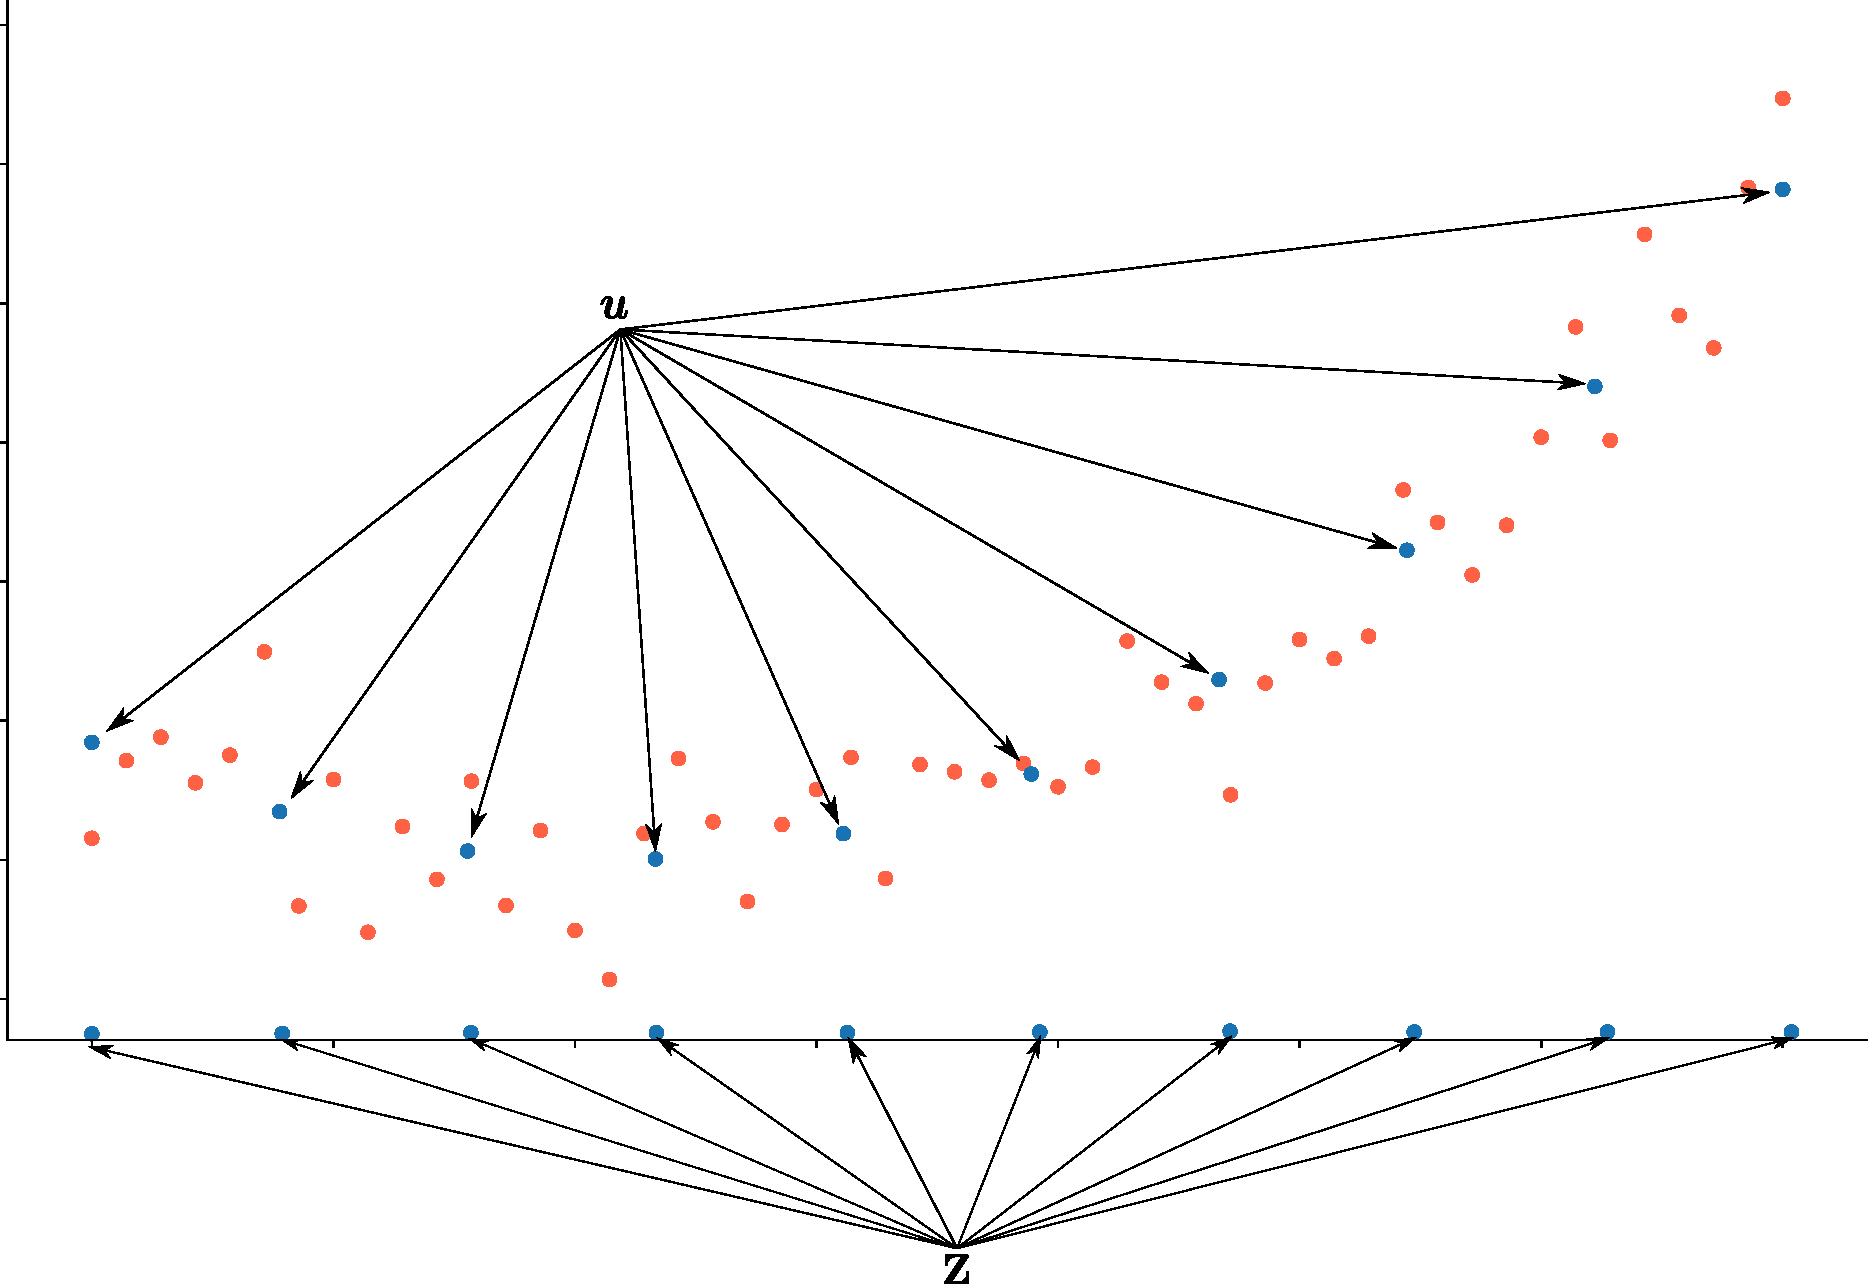
\includegraphics[width=0.7\textwidth]{slides_imgs/GP_inducing_2.pdf}
    \end{center}
    \end{frame}

    \begin{frame}{Sparse Variational Gaussian Processes}
    \begin{center}
    The inducing points can be marginalized in closed form to make predictions.
    \end{center}
    
    \begin{center}
        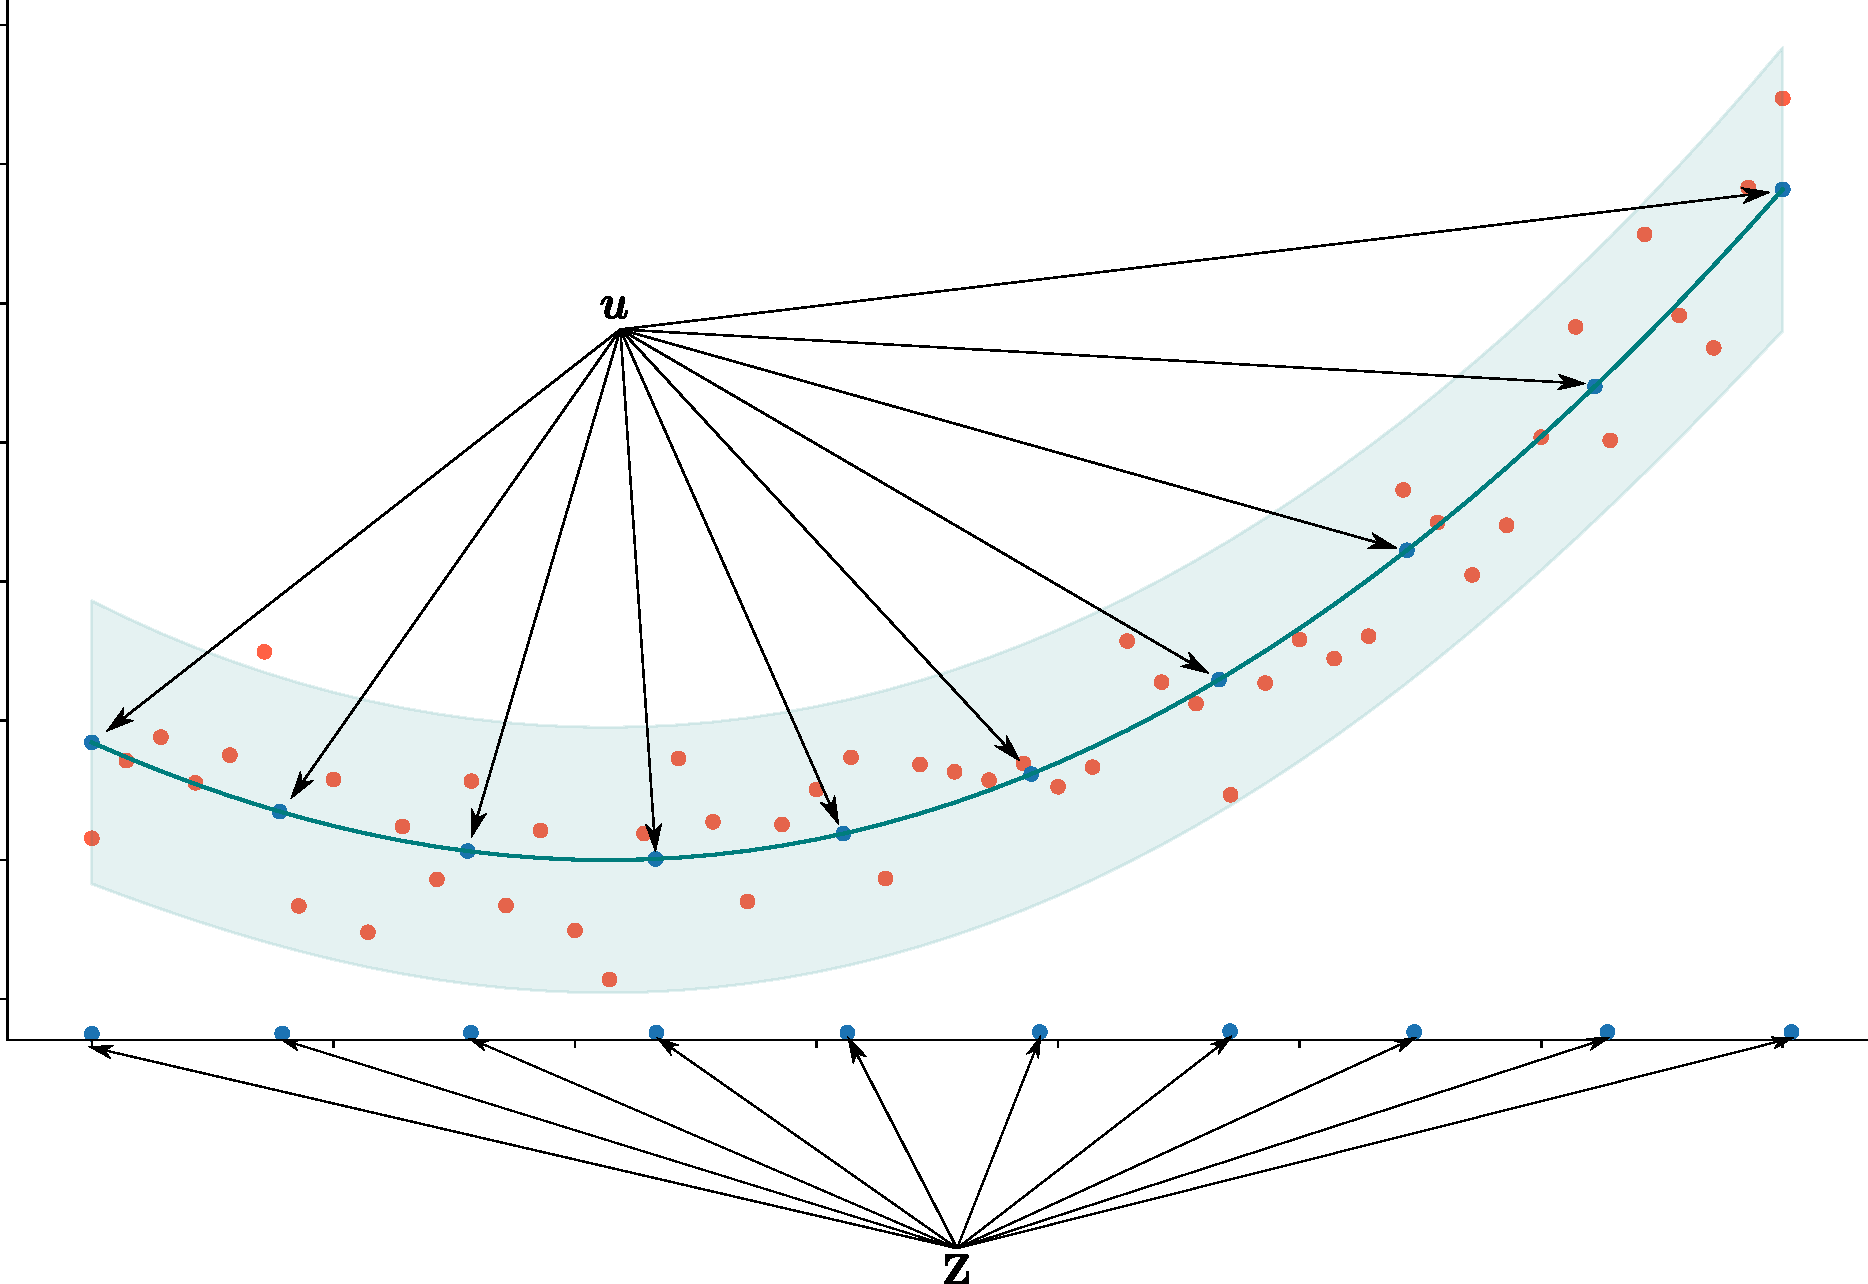
\includegraphics[width=0.7\textwidth]{slides_imgs/GP_inducing_3.pdf}
    \end{center}
    \end{frame}

    \begin{frame}{Hilbert Spaces and RKHS}
        An \textbf{RKHS} \(\mathcal{H}\) is a Hilbert space of functions satisfying the \textbf{reproducing property}: 
        \[
        \forall \mathbf{x} \in \mathcal{X}, \ \exists \phi_{\mathbf{x}} \in \mathcal{H},\quad  \text{such that}\quad \forall g \in \mathcal{H}, \ g(\mathbf{x}) = \braket{\phi_{\mathbf{x}}, g}_\mathcal{H}\,.
        \]
        \pause
         Let \(\mathcal{H}_0(\mathcal{X})\) be the linear span of \(K\) on \(\mathcal{X}\) defined as
        \[
            \mathcal{H}_0(\mathcal{X}) = \Big\{\sum_{i=1}^n a_i K(\cdot, \mathbf{x}_i) \ : \ n \in \mathbb{N}, \ a_i \in \mathbb{R}, \ \mathbf{x}_i \in \mathcal{X}\Big\}\,,
        \]
        by Moore–Aronszajn theorem \(\mathcal{H} := \overline{\mathcal{H}_0(\mathcal{X})}\) is the only Hilbert space verifying the reproducing property as \(\phi_\mathbf{x} = K(\cdot, \mathbf{x}), \ \forall \mathbf{x} \in \mathcal{X}\).
        
                
    \end{frame}
    \begin{frame}{Dual representation of Gaussian Processes}

        Given a \textbf{Gaussian process} \(f\sim \mathcal{GP}(m, K)\), and the RKHS \(\mathcal{H}\) defined by its kernel \(K\). If \(m \in \mathcal{H}\), the GP is equivalent to a Gaussian measure on a Banach space \(\mathcal{B}\) which contains the RKHS \(\mathcal{H}\).
        
        There exists \(\mu \in \mathcal{H}\) and a linear semi-definite positive operator \(\Sigma:\mathcal{H} \to \mathcal{H}\) such that, for any \(\mathbf{x}, \mathbf{x}' \in \mathcal{X}\), \(\exists \phi_{\mathbf{x}}, \phi_{\mathbf{x}'}\in \mathcal{H}\), verifying
        \[
            m(\mathbf{x}) = \braket{\phi_{\mathbf{x}}, \mu}, \quad K(\mathbf{x}, \mathbf{x}') = \braket{\phi_{\mathbf{x}}, \Sigma(\phi_{\mathbf{x}'})}\,.
        \]
        \begin{center}
        \(\mathcal{N}(\mu, \Sigma)\) is a Gaussian measure in \(\mathcal{B}\).
        \end{center}
    {\let\thefootnote\relax\footnote{{CA. Cheng and B. Boots. ``Variational inference for Gaussian process models with linear complexity''}}}
    \end{frame}

    \begin{frame}
        A \textbf{\color{orange}GP prior} is recovered with \(\mu = 0\) and \(\Sigma = I\):
        \[
            m(\mathbf{x}) = \braket{\phi_{\mathbf{x}}, \mu} = 0, \quad K(\mathbf{x}, \mathbf{x}') = \braket{\phi_{\mathbf{x}}, \Sigma(\phi_{\mathbf{x}'})}\,.
        \]
        \pause
        A \textbf{\color{orange}regression GP posterior} is recovered with 
        \[
            \mu = \sum_{i=1}^N \alpha_i \phi_{\mathbf{x}_i} \quad \text{and} \quad \Sigma(\phi)= \phi - \sum_{i=1}^N \sum_{j=1}^N \phi_{\mathbf{x}_i} \Lambda_{i,j} \braket{\phi_{\mathbf{x}_j}, \phi}\,,
        \]
        where \(\bm{\Lambda} = (K(\mathbf{X}, \mathbf{X}) + \sigma^2 \bm{I})^{-1} \in \mathbb{R}^{N \times N}\) and \(\bm{\alpha} = \bm{\Lambda}\bm{y} \in \mathbb{R}^N\).
    \end{frame}

    \begin{frame}
        A SVGP is equivalent to restricting the mean and covariance functions in the RKHS to
        \begin{equation*}
            \tilde{\mu}_{\bm a} = \sum_{m=1}^{M} a_m \phi_{\mathbf{z}_m}\,, \quad \tilde{\Sigma}_{\bm{A}}(\phi) = \phi + \sum_{i=1}^{M}\sum_{j=1}^M\phi_{\mathbf{z}_i} A_{i,j} \braket{\phi_{\mathbf{z}_j}, \phi}\,,
        \end{equation*}
        where \(\bm{a} = (a_1, \dots, a_M)^T \in \mathbb{R}^M\), \(\bm{A} = (A_{ij}) \in \mathbb{R}^{M \times M} \) such that \(\tilde{\Sigma} \geq 0\) and \(\phi_{\mathbf{z}} \in \mathcal{H},\ \forall \mathbf{z} \in \mathbf{Z}\).

     A SVGP with \(q(\mathbf{u})  = \mathcal{N}(\bm \mu, \bm S)\) is \emph{built} with 
     \[
     \bm a = K(\mathbf{Z}, \mathbf{Z})^{-1}\bm \mu\,, \quad
     \bm{A} = K(\mathbf{Z}, \mathbf{Z})^{-1}\bm{S}K(\mathbf{Z}, \mathbf{Z})^{-1} - K(\mathbf{Z}, \mathbf{Z})^{-1}
     \]

    {\let\thefootnote\relax\footnote{{CA. Cheng and B. Boots. ``Variational inference for Gaussian process models with linear complexity''}}}
    \end{frame}

    \begin{frame}
        A SVGP can be \textbf{\color{orange}generalized} with mean and covariance functions of the dual representation in the RKHS to
        \begin{equation*}
        \begin{aligned}
            \tilde{\mu}_{\alpha, \bm a} &= \sum_{m=1}^{M_\alpha} a_m \phi_{\color{red}\mathbf{z}_{\alpha, m}}\\
            \tilde{\Sigma}_{\beta, \bm{A}}(\phi) &= \phi + \sum_{i=1}^{M_ \beta}\sum_{j=1}^{M_\beta}\phi_{\color{blue}\mathbf{z}_{\beta, i}} A_{i,j} \braket{\phi_{\color{blue}\mathbf{z}_{\beta, j}}, \phi}\,.
        \end{aligned}
        \end{equation*}
        where \(\color{red}\mathbf{Z}_\alpha\) and \(\color{blue}\mathbf{Z}_\beta\) are two sets of inducing locations.
        
    {\let\thefootnote\relax\footnote{{CA. Cheng and B. Boots. ``Variational inference for Gaussian process models with linear complexity''}}}
    \end{frame}
    \begin{frame}{Fixing the Mean Function}
            Let \(\mathcal{Z} \subset \mathcal{X}\) any compact subset of the input space. If the kernel is \textbf{\color{orange}universal}, for any function \(h \in C(\mathcal{Z})\) and \(\epsilon > 0 \), there exists \(M_\alpha > 0\), a set of inducing locations \(\{\mathbf{z}_1, \dots, \mathbf{z}_{M_\alpha}\} \subset \mathcal{Z}\), and scalar values \(a_1, \dots, a_{M_\alpha}\) such that
            \[
                m(\mathbf{x}) = \braket{\phi_{\mathbf{x}}, \tilde{\mu}_{\alpha, \bm{a}}} = \sum_{m=1}^{M_\alpha}a_m K(\mathbf{x}, \mathbf{z}_m) 
            \]
            verifies
            \[
            \big\|h(\mathbf{x}) -  m(\mathbf{x})\big\|_{\mathcal{Z}} \leq \epsilon\,.
            \]
    \end{frame}
\begin{frame}
        \begin{center}
            \textbf{Distributions over function-space with fixed mean to \(h\).}
        \end{center}
        \pause
        \begin{center}
        \textbf{Parameters}: \(\mathbf{Z}_{\beta} \subset \mathbb{R}^D\) and \(\bm{A} \in \mathbb{R}^{M_\beta \times M_\beta}\) (such that \(\tilde{\Sigma} \geq 0\)).
        \end{center}
        \pause
        \begin{center}  
        Gaussian process posterior approximation \(\mathcal{GP}(m^\star, K^\star)\):
        \end{center}
        \[
            \begin{aligned}
                m^{\star}(\mathbf{x}) &\approx h(\mathbf{x})\,, \\
                K^{\star}(\mathbf{x}, \mathbf{x}') &=K(\mathbf{x}, \mathbf{x}') +  K(\mathbf{x}, \mathbf{Z}_\beta)\bm{A}^{-1} K(\mathbf{Z}_\beta, \mathbf{x}')\,,
            \end{aligned}
        \]
    \end{frame}

    \begin{frame}{Diagram - Distribution over function-space}
        \begin{figure}[h]
        	\begin{center}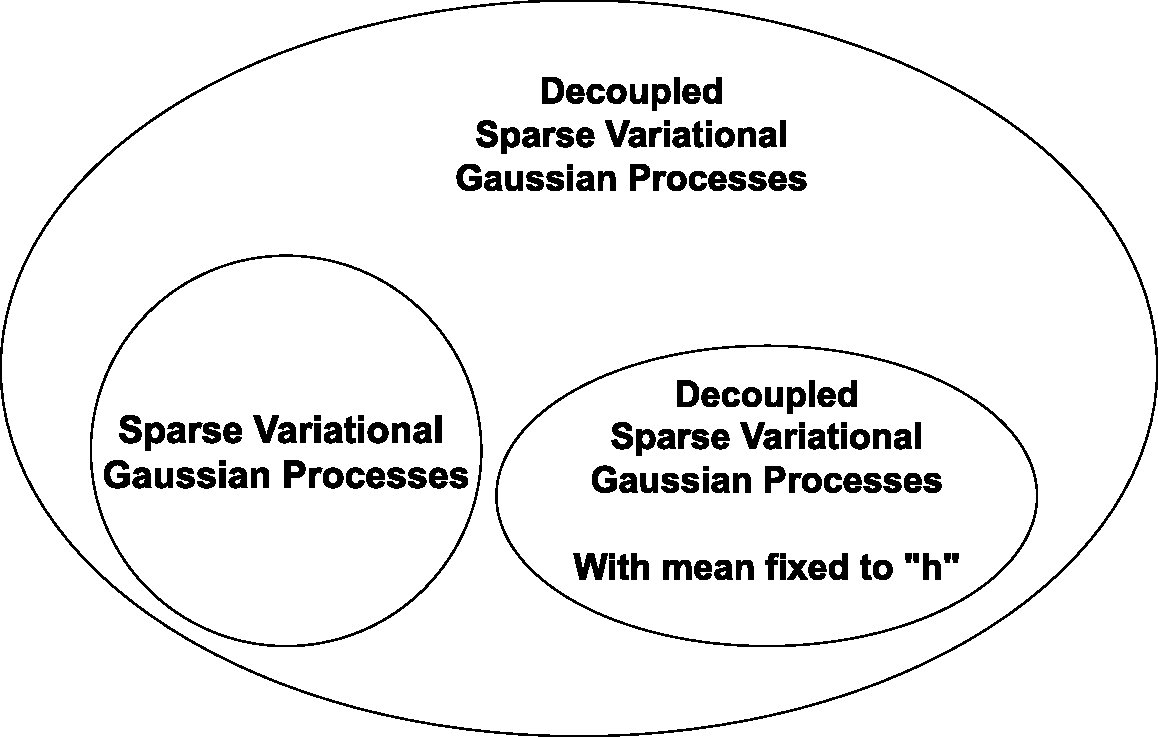
\includegraphics[width=0.90\textwidth]{slides_imgs/diagram.pdf} 
        	\end{center}
        \end{figure}
    \end{frame}
    \begin{frame}{Diagram - Distribution over function-space}
        \begin{figure}[h]
        	\begin{center}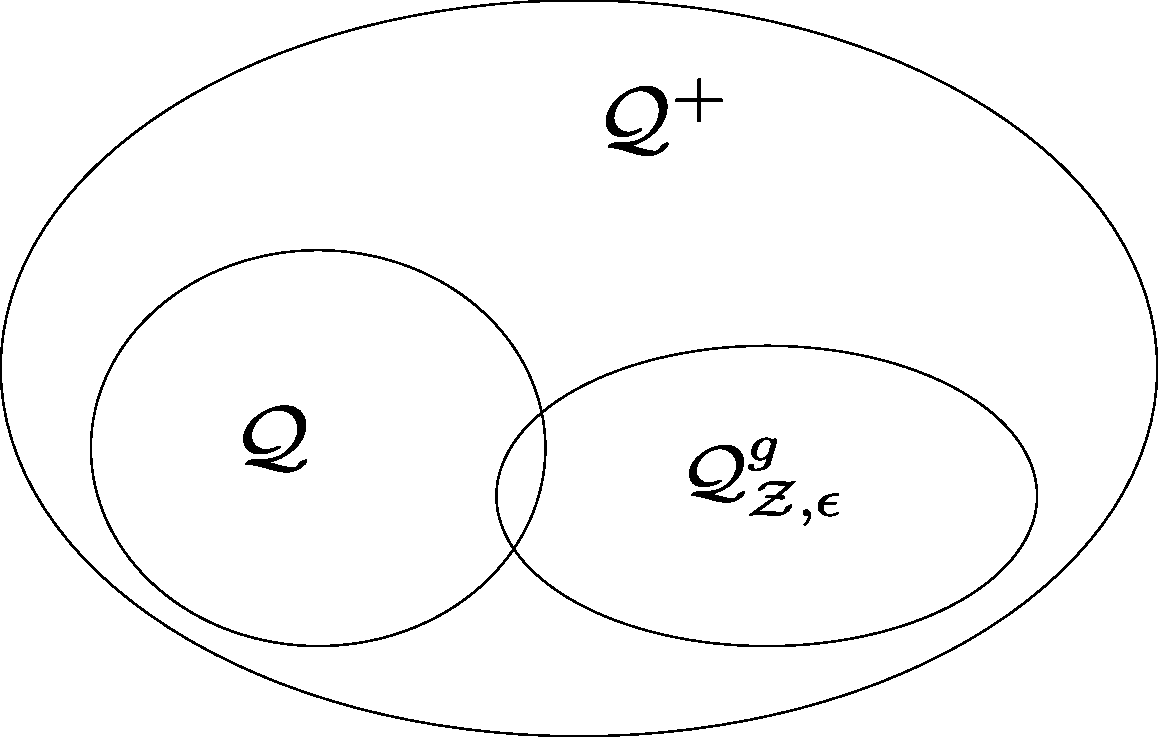
\includegraphics[width=0.90\textwidth]{slides_imgs/diagram2.pdf} 
        	\end{center}
        \end{figure}
    \end{frame}
    \begin{frame}{Variational Inference in Different Families}
        \begin{center}
            \textbf{Sparse Variational Gaussian Processes}
        \end{center}
        \[
        q^\star = \argmax_{q \in \mathcal{Q}}\  \mathbb{E}_{q(f)}[ \log p(\mathbf{y} | f)] - \text{KL}\big(q|p\big)
        \]   
        \pause
        \begin{center}
            \textbf{Decoupled Sparse Variational Gaussian Processes}
        \end{center}
        \[
        q^\star = \argmax_{q \in {\color{red}\mathcal{Q}^+}}\ \mathbb{E}_{q(f)}[ \log p(\mathbf{y} | f)] - \text{KL}\big(q|p\big)
        \]   
        \pause
        \begin{center}
            \textbf{Fixed Mean Sparse Variational Gaussian Processes}
        \end{center}
        \[
        q^\star = \argmax_{q \in {\color{red}\mathcal{Q}^h}}\  \mathbb{E}_{q(f)}[ \log p(\mathbf{y} | f)] - \text{KL}\big(q|p\big)
        \]   
    \end{frame}

    \begin{frame}{Variational Optimization}
        Optimizing the ELBO in the Hilbert space:
        \[
        q^\star = \argmax_{q \in \mathcal{Q}}\ \mathbb{E}_{q(f)} \left[ \log p(\mathbf{y}|f)\right] - \text{KL}\left(q|p\right)\,.
        \]
        Where
        \[
            \text{KL}\left(q | p\right) = \frac{1}{2} \bm{a}^T \bm{K}_{\bm Z} \bm{a} +  \frac{1}{2} \log |\bm{I} - \bm{K}_{\bm{Z}} (\bm{A} + \bm{K}_{\bm{Z}})^{-1}| + \frac{1}{2} \text{tr}\left( \bm{K}_{\bm{Z}}\bm{A}^{-1} \right)
        \]
        and \(\mathbb{E}_{q(f)}\left[ \log p(\mathbf{y}|f)\right] \) can be computed in regression and estimated in classification.
    \end{frame}
    
    \begin{frame}{Variational Optimization}
        Optimizing the ELBO in the Hilbert space:
        \[
        q^\star = \argmax_{q \in {\color{red}\mathcal{Q}^+}}\ \mathbb{E}_{q(f)} \left[ \log p(\mathbf{y}|f)\right] - \text{KL}\left(q|p\right)\,.
        \]
        where
        \[
            \text{KL}\left(q | p\right) = \underbrace{\frac{1}{2} \bm{a}^T \bm{K}_{\alpha} \bm{a}}_{\bm{a}, \mathbf{Z}_\alpha} +  \underbrace{\frac{1}{2} \log |\bm{I} - \bm{K}_{\beta} (\bm{A} + \bm{K}_{\beta})^{-1}| + \frac{1}{2} \text{tr}\left( \bm{K}_\beta\bm{A}^{-1} \right)}_{\bm{A}, \mathbf{Z}_\beta}
        \]
        and \(\mathbb{E}_{q(f)}\left[ \log p(\mathbf{y}|f)\right] \) can be computed in regression and estimated in classification.
    \end{frame}

    \begin{frame}{Variational Optimization}
        Optimizing the ELBO in the Hilbert space:
        \[
        q^\star = \argmax_{q \in {\color{red}\mathcal{Q}^h}}\ \mathbb{E}_{q(f)} \left[ \log p(\mathbf{y}|f)\right] - \text{KL}\left(q| p\right)\,.
        \]
        where
        \[
            \begin{aligned}
                \text{KL}\left(q | p\right) = \frac{1}{2} {\color{red}\bm{a}^T \bm{K}_{\alpha} \bm{a}} + \frac{1}{2} \log |\bm{I} - \bm{K}_{\beta} (\bm{A} + \bm{K}_{\beta})^{-1}| + \frac{1}{2} \text{tr}\left( \bm{K}_\beta\bm{A}^{-1} \right)
            \end{aligned}
        \]
        and \(\mathbb{E}_{q(f)}\left[ \log p(\mathbf{y}|f)\right] \) can be computed in regression and estimated in classification.
    \end{frame}

    \begin{frame}{Intuitive Recap}
        \begin{enumerate}[<+->]\color{shadecolor}
            \item \color<.>{black}Learn a \textbf{optimal deterministic} model \(h\).
            \item \color<.>{black}Define a \textbf{Sparse Variational GP}.
            \item \color<.>{black}\textbf{Decouple the inducing locations} from the mean and covariance.
            \item \color<.>{black}Consider the \textbf{subspace with fixed mean} \(h\).
            \item \color<.>{black}Train the (non-fixed) parameters using \textbf{function-space VI} and mini-batch optimization.
            \item \color<.>{black}The resulting method \textbf{provides uncertainty estimation} for the deterministic model.
        \end{enumerate}
    \end{frame}
    
    \begin{frame}{Results in Regression Problems}
    \begin{figure}
        \centering
        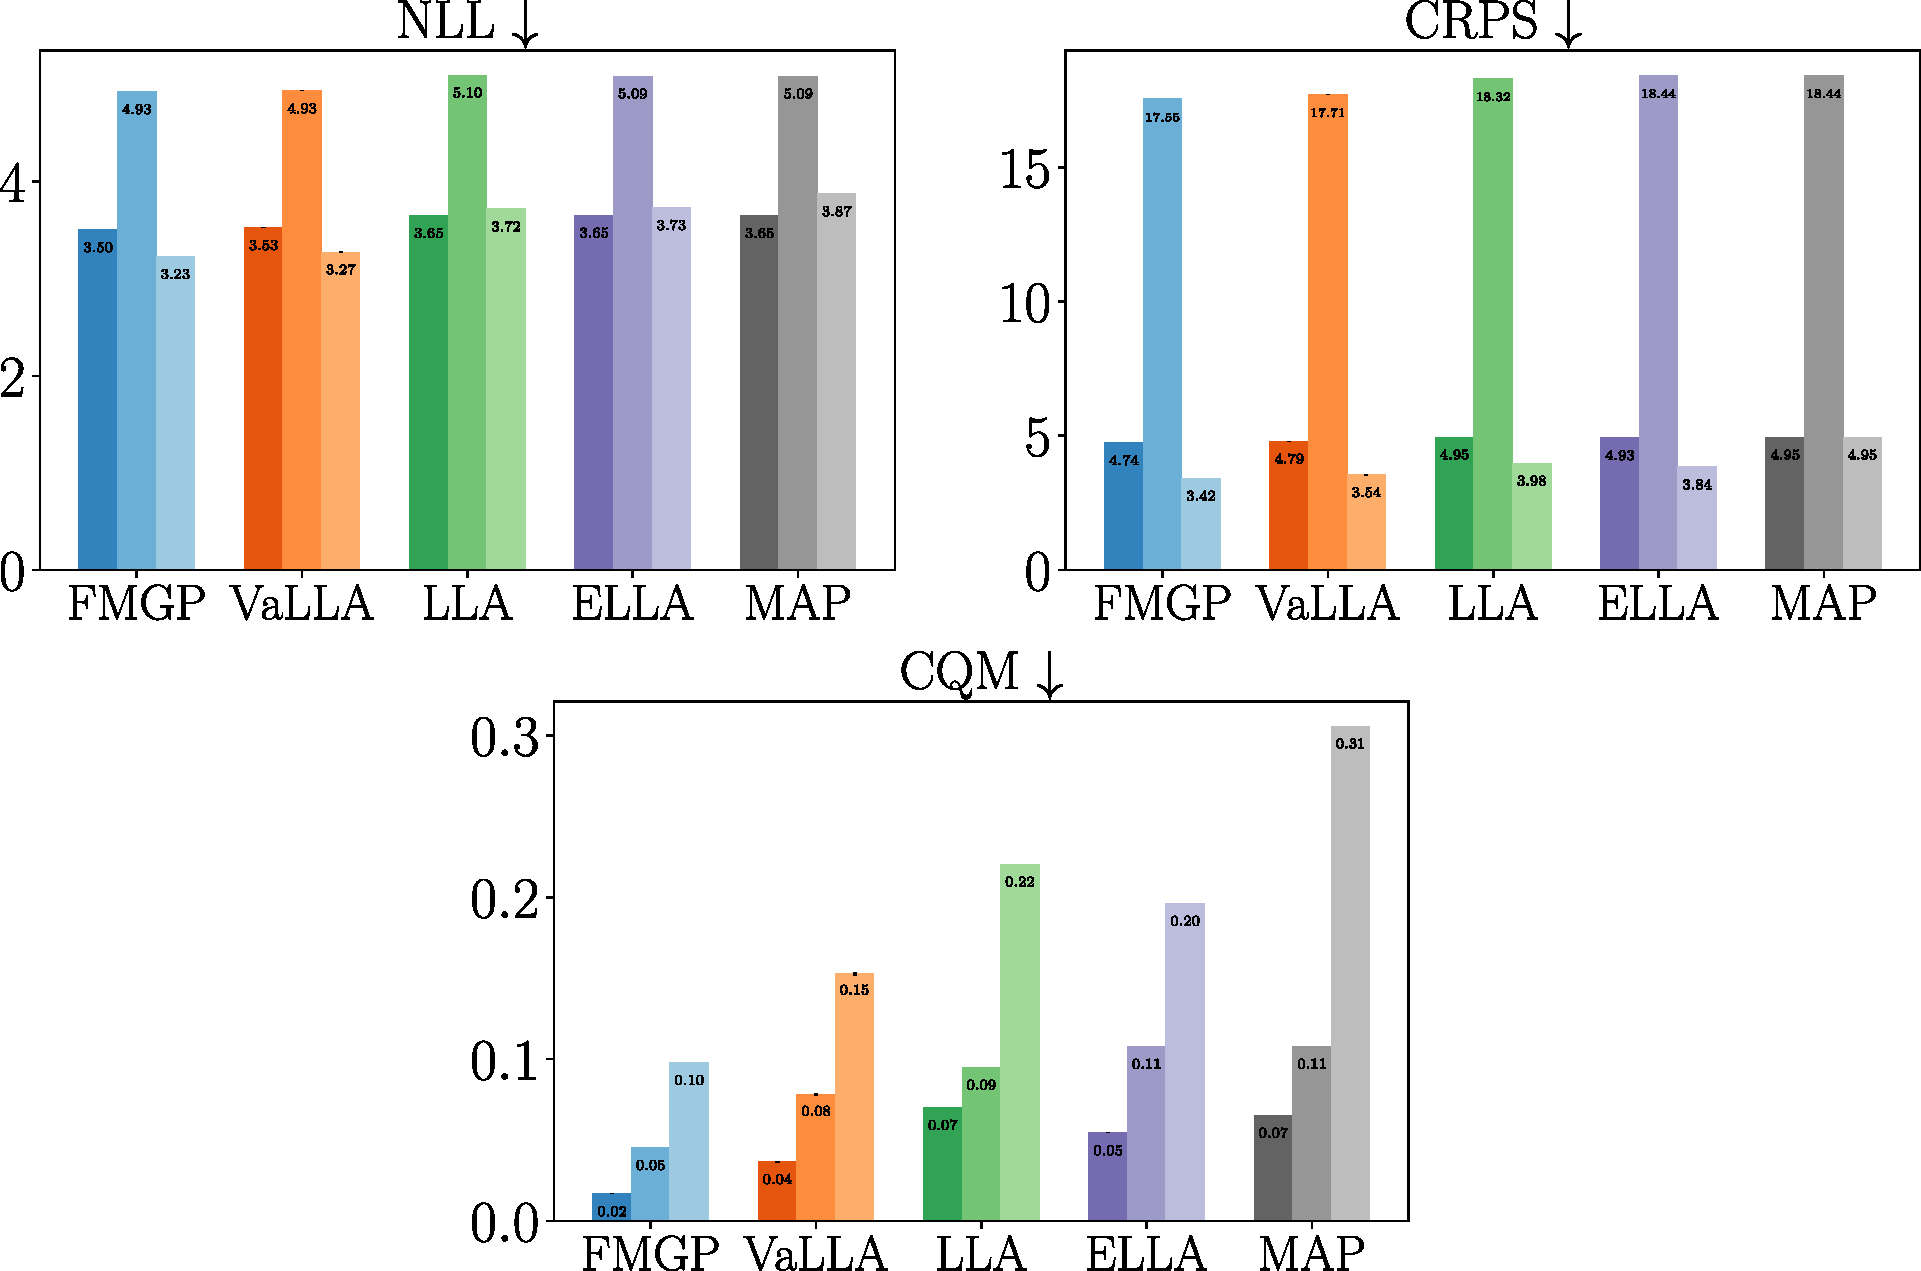
\includegraphics[width=0.9\linewidth]{slides_imgs/regression_3.pdf}
        \caption{Caption}
        \label{fig:enter-label}
    \end{figure}
    \end{frame}

    
    {\setbeamercolor{background canvas}{bg=white}
    \begin{frame}{Results in Cifar10 Problems}
        \centering
        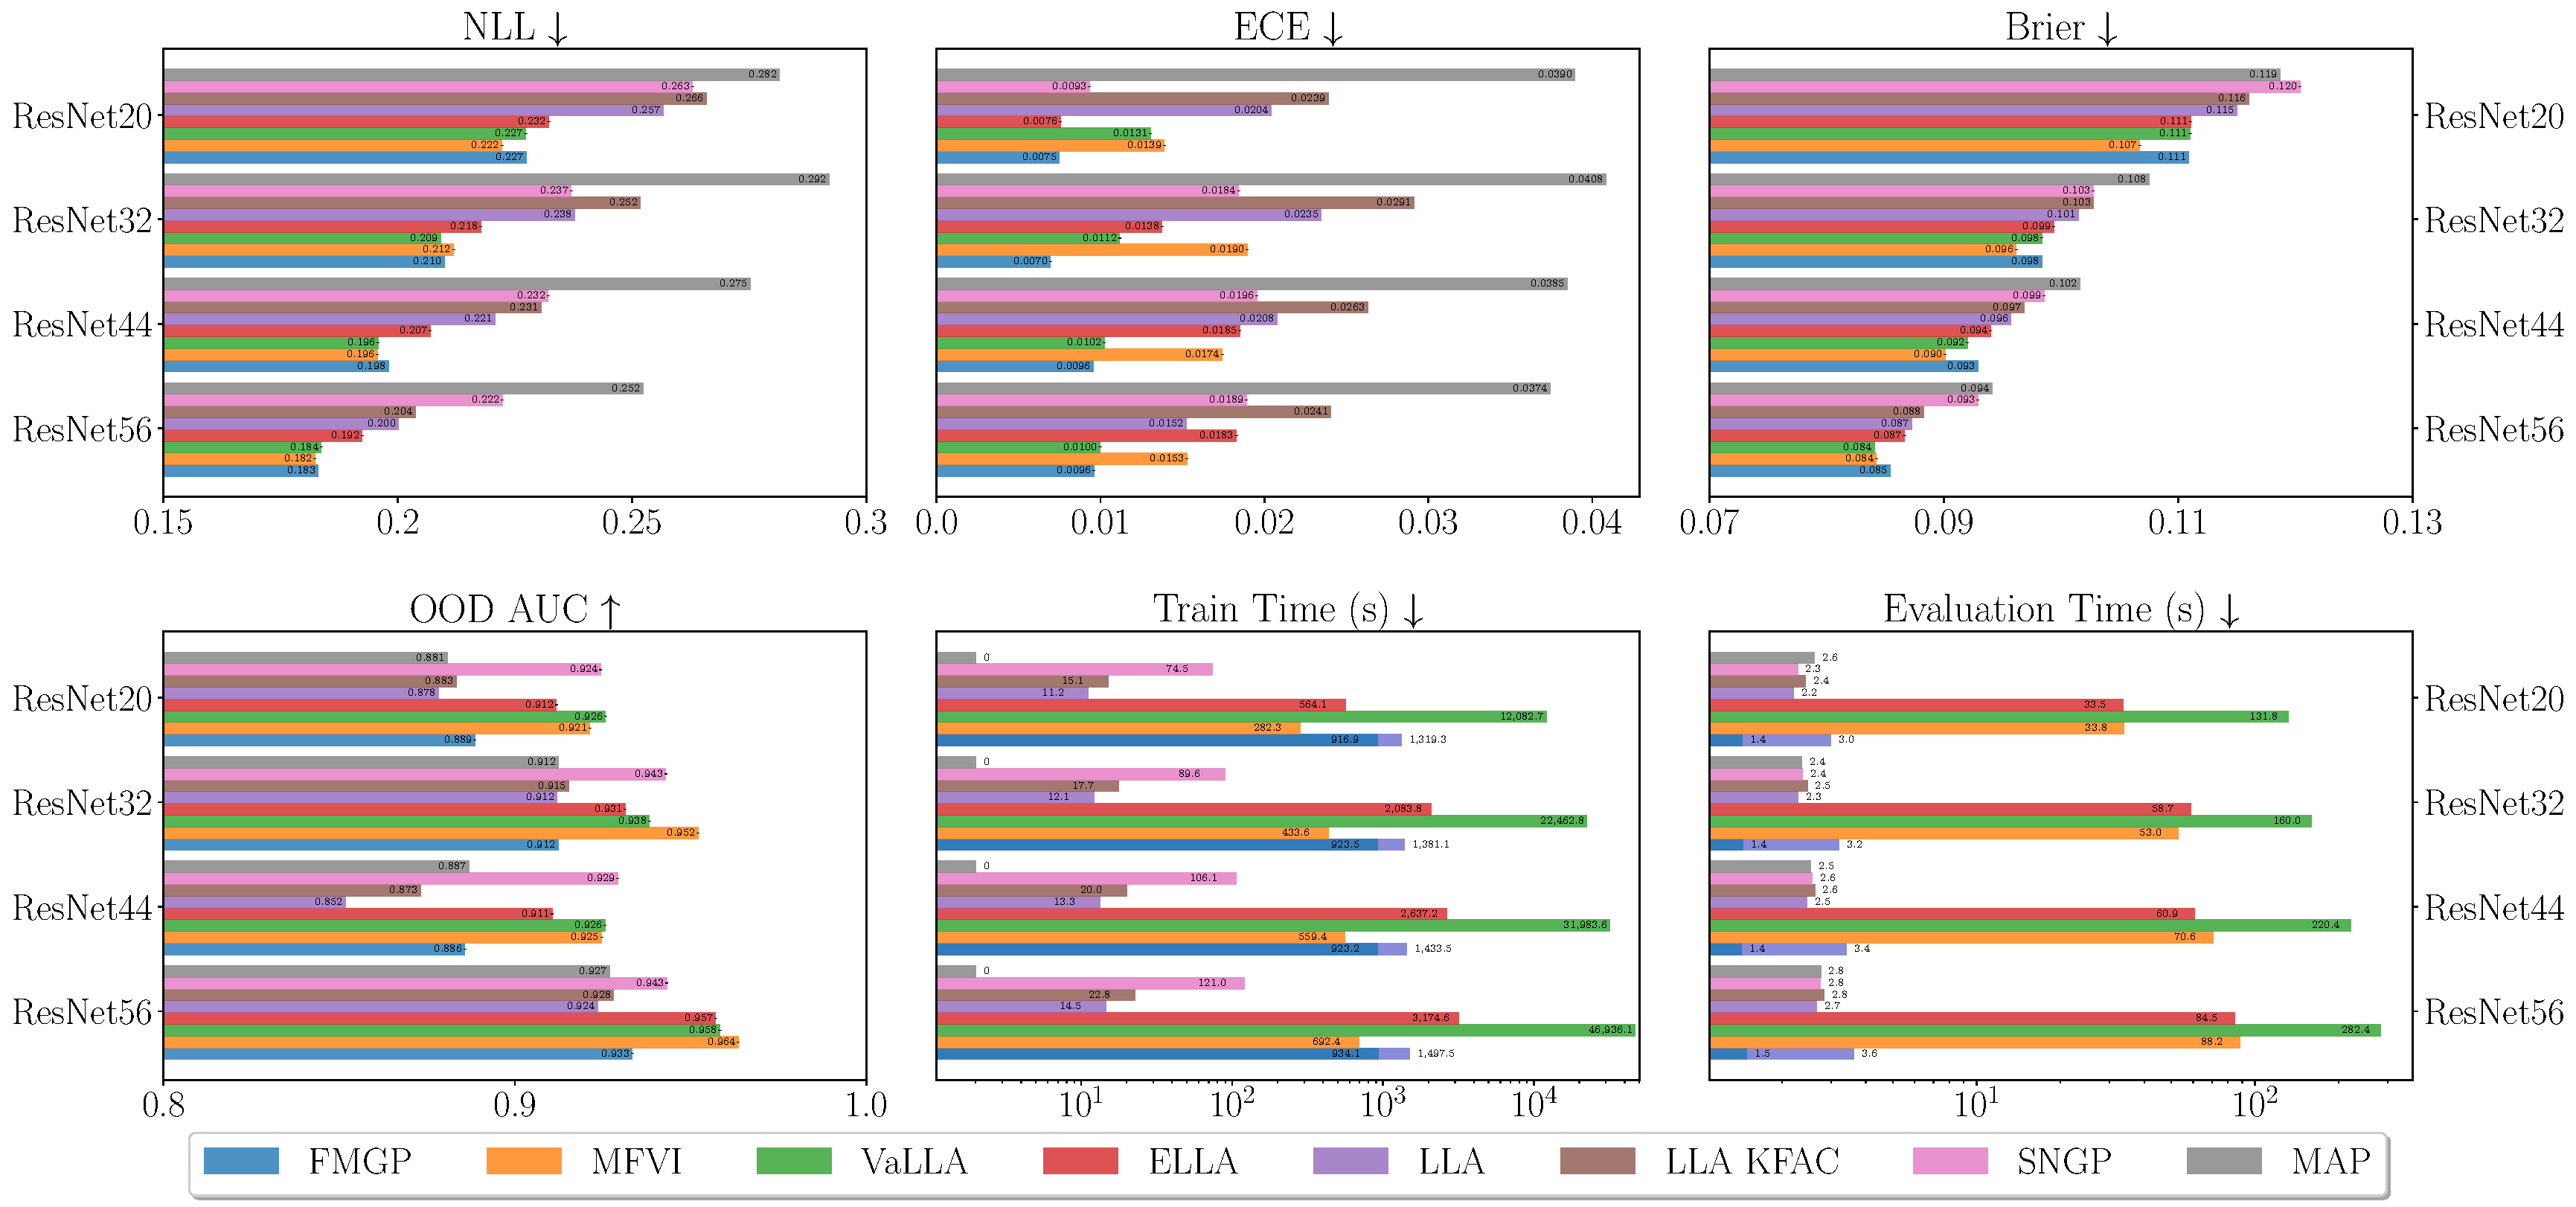
\includegraphics[width=1\linewidth]{slides_imgs/cifar10.pdf}
    \end{frame}}

    \begin{frame}{Results in Imagenet}
    \begin{table}[ht]
    \centering
    \scalebox{0.65}{
    \begin{tabular}{llcccccc}
        \hline
        \textbf{Model} & \textbf{Method} & \textbf{NLL} & \textbf{ECE} & \textbf{Train Time} & \textbf{Test Time} \\
        \hline
        \multirow{4}{*}{ResNet18}  & MAP & {\color{teal}$\mathbf{1.247 \pm 0.000}$} & $0.026 \pm 0.000$ & {\color{purple}$\mathbf{0.000 \pm 0.000}$} & {\color{purple}$\mathbf{5.058 \pm 0.029 \times 10^2}$} \\
        & ELLA & $1.248 \pm 0.000$ & {\color{teal}$\mathbf{0.025 \pm 0.000}$} & {\color{teal}$\mathbf{7.890 \pm 0.275 \times 10^3}$} & $8.060 \pm 0.010 \times 10^2$ \\
        & FMGP & $1.248 \pm 0.001$ & {\color{purple}$\mathbf{0.015 \pm 0.001}$} & $1.835 \pm 0.099 \times 10^4$ & {\color{teal}$\mathbf{7.324 \pm 0.001 \times 10^2}$} \\
        & MFVI & {\color{purple}$\mathbf{1.242 \pm 0.001}$} & $0.040 \pm 0.000$ & $7.602 \pm 0.032 \times 10^4$ & $3.773 \pm 0.308 \times 10^4$ \\
        \hline
        \multirow{3}{*}{ResNet34}  & MAP & {\color{teal}$\mathbf{1.081 \pm 0.000}$} & $0.035 \pm 0.000$ & {\color{purple}$\mathbf{0.000 \pm 0.000}$} & {\color{purple}$\mathbf{5.088 \pm 0.004 \times 10^2}$} \\
        & ELLA & $1.082 \pm 0.000$ & {\color{teal}$\mathbf{0.034 \pm 0.000}$} & {\color{teal}$\mathbf{1.201 \pm 0.373 \times 10^4}$} & $1.087 \pm 0.018 \times 10^3$ \\
        & FMGP & {\color{purple}$\mathbf{1.077 \pm 0.000}$} & {\color{purple}$\mathbf{0.016 \pm 0.000}$} & $1.942 \pm 0.103 \times 10^4$ & {\color{teal}$\mathbf{8.563 \pm 0.011 \times 10^2}$} \\
        \hline
        \multirow{3}{*}{ResNet50} & MAP & {\color{teal}$\mathbf{0.962 \pm 0.000}$} & $0.037 \pm 0.000$ & {\color{purple}$\mathbf{0.000 \pm 0.000}$} & {\color{purple}$\mathbf{4.954 \pm 0.010 \times 10^2}$} \\
        & ELLA & {\color{teal}$\mathbf{0.962 \pm 0.000}$} & {\color{teal}$\mathbf{0.036 \pm 0.000}$} & $2.997 \pm 1.215 \times 10^4$ & $1.954 \pm 0.018 \times 10^3$ \\
        & FMGP & {\color{purple}$\mathbf{0.958 \pm 0.001}$} & {\color{purple}$\mathbf{0.018 \pm 0.001}$} & {\color{teal}$\mathbf{2.543 \pm 0.046 \times 10^4}$} & {\color{teal}$\mathbf{1.100 \pm 0.010 \times 10^3}$} \\
        \hline
        \multirow{3}{*}{ResNet101} & MAP & {\color{teal}$\mathbf{0.912 \pm 0.000}$} & $0.049 \pm 0.000$ & {\color{purple}$\mathbf{0.000 \pm 0.000}$} & {\color{purple}$\mathbf{5.059 \pm 0.001 \times 10^2}$} \\
        & ELLA & $0.913 \pm 0.000$ & {\color{teal}$\mathbf{0.048 \pm 0.000}$} & $4.464 \pm 1.649 \times 10^4$ & $2.808 \pm 0.001 \times 10^3$ \\
        & FMGP & {\color{purple}$\mathbf{0.900 \pm 0.000}$} & {\color{purple}$\mathbf{0.030 \pm 0.001}$} & {\color{teal}$\mathbf{2.654 \pm 0.064 \times 10^4}$} & {\color{teal}$\mathbf{1.134 \pm 0.001 \times 10^3}$} \\
        \hline
        \multirow{3}{*}{ResNet152} & MAP & {\color{teal}$\mathbf{0.876 \pm 0.000}$} & $0.050 \pm 0.000$ & {\color{purple}$\mathbf{0.000 \pm 0.000}$} & {\color{purple}$\mathbf{6.324 \pm 0.004 \times 10^2}$} \\
        & ELLA & $0.877 \pm 0.000$ & {\color{teal}$\mathbf{0.048 \pm 0.000}$} & $6.820 \pm 0.526 \times 10^4$ & $3.877 \pm 0.007 \times 10^3$ \\
        & FMGP & {\color{purple}$\mathbf{0.865 \pm 0.001}$} & {\color{purple}$\mathbf{0.024 \pm 0.001}$} & {\color{teal}$\mathbf{2.973 \pm 0.069 \times 10^4}$} & {\color{teal}$\mathbf{1.267 \pm 0.002 \times 10^3}$} \\
        \hline
    \end{tabular}}
\end{table}
        
    \end{frame}

    \begin{frame}{Results on Molecular Property Prediction}
        \begin{table}[]
        \centering
        \begin{tabular}{lcc}
        \hline
        \textbf{Method} & \textbf{NLL} & \textbf{CRPS} \\\hline
        MAP & \(-1.76 \pm 0.016\) & \(0.0221 \pm 0.00\) \\    
        LLA & \(-1.78 \pm 0.021\) & {\color{teal}$\mathbf{0.0218 \pm 0.00}$}  \\
        ELLA & {\color{teal}$\mathbf{-1.80 \pm 0.013}$}  & $0.0219 \pm 0.00$ \\
        FMGP & {\color{purple}$\mathbf{-1.85 \pm 0.017}$} & {\color{purple}$\mathbf{0.0216 \pm 0.00}$} \\
        \hline
        \end{tabular}
        \caption{Results on QM9 dipole moment prediction task.}
        \label{tab:qm9}
        \end{table}
    \end{frame}

    \begin{frame}{Conclusions}
        \begin{enumerate}[<+->]
            \item Sparse GPs can be \textbf{characterized} in the RKHS.
            \item Sparse GPs can be generalized to \textbf{decouple the inducing points}.
            \item There exists a \textbf{subspace} with posterior mean \(h\).
            \item Obtained results are promising.
        \end{enumerate}
    \end{frame}

    \begin{frame}[standout]
        Thank you for your attention!
    \end{frame}
    \begin{frame}{Dual representation of Gaussian Processes}

        A \textbf{Gaussian process} \(f\sim \mathcal{GP}(m, K)\) has a \textbf{\color{orange}dual representation} in a RKHS \(\mathcal{H}\) \emph{from a {\color{orange}different unknown} kernel \(\tilde{K}\)}.
        
        There exists \(\mu \in \mathcal{H}\) and a linear semi-definite positive operator \(\Sigma:\mathcal{H} \to \mathcal{H}\) such that, for any \(\mathbf{x}, \mathbf{x}' \in \mathcal{X}\), \(\exists \phi_{\mathbf{x}}, \phi_{\mathbf{x}'}\in \mathcal{H}\), verifying
        \[
            m(\mathbf{x}) = \braket{\phi_{\mathbf{x}}, \mu}, \quad K(\mathbf{x}, \mathbf{x}') = \braket{\phi_{\mathbf{x}}, \Sigma(\phi_{\mathbf{x}'})}\,.
        \]
        \begin{center}
        \(\mathcal{N}(\mu, \Sigma)\) is a Gaussian measure in \(\mathcal{H}\).
        \end{center}
    {\let\thefootnote\relax\footnote{{I. Holmes and A. N. Sengupta, ``The Gaussian radon transform and machine learning''\\CA. Cheng and B. Boots, ``Incremental variational sparse Gaussian process regression''}}}
    \end{frame}
    \begin{frame}{Regularization}
         In standard sparse GPs, tuning hyper-parameters involves \textbf{balancing} the fit of the mean to training data against reducing the model's predictive variance. 

         
        We consider another Gaussian measure \(q^\star \in \mathcal{Q}\) that shares \(q\)'s parameters but also incorporates \(\bm{a} \in \mathbb{R}^{M_\beta}\) and \(\mathbf{Z} = \mathbf{Z}_\beta\) as additional parameters for its predictive mean.
         \[
            \begin{aligned}
            \mathcal{L}(\bm{a}, \bm{A}, \mathbf{Z}, \theta) &= \underbrace{\mathbb{E}_{q(f)}[\log p(\mathbf{y}|f)] - \text{KL}\big(q \big| p\big)}_{\text{ELBO}(q)} \\
            &\quad + \underbrace{\mathbb{E}_{q^\star(f)}[\log p(\mathbf{y}|f)] - \text{KL}\big(q^\star \big| p\big)}_{\text{ELBO}(q^\star)}
            \end{aligned}
            \]
    \end{frame}
\end{document}